\documentclass[finnish]{tktltiki2}
\usepackage[utf8]{inputenc}
\usepackage[T1]{fontenc}
\usepackage{amsfonts,amsmath,amssymb,amsthm,booktabs,color,enumitem,graphicx}
\usepackage[pdftex,hidelinks]{hyperref}

\makeatletter
\AtBeginDocument{\hypersetup{pdftitle = {\@title}, pdfauthor = {\@author}}}
\makeatother

\usepackage[fixlanguage]{babelbib}
\selectbiblanguage{finnish}

%\doublespacing
%\singlespacing
%\onehalfspacing

\title{Mutaatiotestaus -- working title}
\author{Tony Kovanen}
\date{\today}
\abstract{Tiivistelmä.}
\level{Kandidaatintutkielma}
\keywords{Ohjelmistojen testaus, mutatointi}

\begin{document}

\frontmatter

\maketitle
\makeabstract

\tableofcontents
\newpage

\section{Johdanto}
Ohjelmistoja tuotettaessa on tärkeää varmistaa ohjelmiston eri komponenttien toimivuus ja niiden yhteensopivuus. Toimivuus varmistetaan usein automaattisella ohjelmistojen testaamisella. Testauksen rooli ohjelmistotuotantoprosessissa vie potentiaalisesti paljon resursseja suhteessa itse tuotteen toteutukseen, mutta se myös torjuu tehokkaasti viallista ja bugista koodia~\cite{SchulerZ10}. Vaikka testaus ei anna täysin objektiivista totuutta siitä, toimiiko ohjelmisto kuten on odotettu, tai täsmälleen sille asetettujen vaatimusten mukaan, se kasvattaa ohjelmoijien luottamusta tuotteen laatuun. Kattavien testien läsnäollessa voidaan myös huoletta lisätä uusia toiminnallisuuksia ohjelmistoon ja refaktoroida ohjelmakoodia, eli parannella olemassaolevaa koodia ja ohjelman rakennetta, sillä epäonnistuvat testit huomauttavat vanhan toiminnallisuuden tai komponenttien yhteensopivuuden rikkomisesta. 

Yksittäisten komponenttien automatisoitu testaaminen voidaan tehdä yksikkötesteillä. Niillä voidaan varmistaa olio-ohjelmointikielissä yksittäisten luokkien ja niiden metodien toimivuus. Vastaavia testejä voidaan kirjoittaa myös esimerkiksi funktionaalisilla ohjelmointikielillä, joissa yksikkötestit testaavat yksittäisten funktioiden ja moduulien (jos ne sisältyvät ohjelmointikieleen) toiminnallisuutta. Yksikkötestit antavat välitöntä palautetta siitä, toimiiko muutoksen kohteena oleva komponentti edelleen olennaisesti samalla tavalla kuin aiemmin. Yksikkötesteillä tulee usein testattua myös jossain määrin komponenttien yhteistoimintaa, sillä oliot usein kapseloivat sisäänsä toisia olioita, jolloin testattavan olion toimivuus riippuu sen kapseloimien olioiden toimivuudesta. 

Integraatiotesteillä testataan komponenttien toimivuus yhdessä tarkemmin ja kattavemmin. Tämä tapahtuu usein simuloimalla kokonaisia ohjelmiston toimintoja. Järjestelmätestit ovat käyttäjätason testejä, joilla ohjelmistolle suoritetaan kokonainen käyttäjän toiminto, jonka tulos evaluoidaan. 

%Tässä tutkielmassa keskitytään yksikkötestien kattavuuden mittaamiseen. Kattavuutta voidaan mitata yleistämällä erilaisia kattavuusmittoja helposti myös esimerkiksi integraatiotesteille. 

Niin yksikkö- kuin integraatiotestien yhteydessä puhutaan usein testauskattavuudesta. Ideaalisesti se, että jotkin testit kattavat ohjelman, tarkoittaa sitä, että virheellinen ohjelma huomataan yhden tai useamman testin epäonnistuessa. Kattavuuden mittana tunnetuimmat ja yleisimmät ovat rivikattavuus ja haarautumakattavuus. Näitä kattavuusmetriikoita tarjoavat useimmat testauskattavuustyökalut. Kuten huomaamme pian, nämä kattavuusmetriikat eivät ole täysin ideaalisen määritelmän mukaisia.

Rivikattavuudessa tarkastellaan, millä annetun ohjelman riveillä käydään testejä suoritettaessa. Jos testien suorituksen käydään jokaisella ohjelmakoodin rivillä, on testikattavuus 100\%. Käytännössä rivikattavuus lasketaan siis kaavalla $\frac{\text{suoritetut rivit}}{\text{rivien määrä}}$.

Haarautumakattavuus mittaa eri kontrollirakenteista syntyvien haarautumien kattavuuden, eli se kertoo prosentuaalisesti sen määrän eri kontrollihaaroista, minkä ohjelmakoodin testit ovat suorittaneet testattavasta komponentista. Useimmat testauskattavuustyökalut tarjoavat molemmat näistä kattavuusmetriikoista. Jotkut työkalut tarjoavat myös ehtokattavuuden, eli mitan siitä, kuinka moni totuusarvo on evaluoitunut sekä todeksi että epätodeksi.

Rivi- ja haarakattavuutta saadaan lisättyä testeillä, jotka eivät välttämättä edes testaa mitään. Kattavuuksien arvot kasvavat kun useampi rivi suoritetaan ohjelmakoodista, joten nämä metriikat eivät takaa mitään ohjelman laadukkuudesta. Mutaatiokattavuus on eräs metriikka, jolla pyritään semanttisempaan analyysin testien kattavuudesta. Mutaatiotestauksen tavoite on saada selville, kuinka kattavasti määritellyt testit löytävät ohjelmakoodiin tuotettavia pieniä mahdollisia bugeja simuloivia muutoksia. Mutaatiokattavuuden kattavuusmitta suurenee vain kun testit huomaavat useampia mahdollisia bugeja antaen joitain takeita siitä, että mutaatiotestauksella saadaan tuotettua virheettömämpiä ohjelmistoja.

Kaikista kattavuuksista on usein tarjolla pelkän metriikan tuottaman kattavuusluvun lisäksi myös raportti, josta kattavuuden ulkopuolelle jäävät rivit ja haarat tulevat esille. Myös useat mutaatioanalyysiä tukevat testikehykset näyttävät vastaavanlaisen raportin, jossa ohjelmoijalle näytetään se osa koodista, johon tehtyä muutosta ei havaittu sille kirjoitetuilla testeillä. Näistä raporteista löytyy esimerkkejä tutkielman lopussa. Tutkielmassa keskitytään yksikkötestien kattavuuden mittaamiseen, erityisesti mutaatiotestaukseen, sen hyötyihin ja ongelmiin. Tutkielmassa esitetyt konseptit ovat kuitenkin helposti yleistettävissä esimerkiksi integraatiotesteille.

\section{Mutaatiotestaus}
Mutaatiotestauksessa pyritään löytämään ohjelman mahdollisten syötteiden rajatapauksia, joita testikehykselle annetut testit eivät kata ja näiden avulla parannella ohjelmaa lopulta saavuttaen toivottavasti ideaalisen testikattavuuden. Mutaatiotestaus tapahtuu ohjelmalle suoritettavalla testaussyklillä. Ensin ohjelman testit ajetaan alkuperäiselle lähdekoodille. Jos jokin testi epäonnistuu, se tulee korjata ennen jatkamista. Tarve tähän tarkistukeen on ilmeinen: jos alkuperäinen ohjelma ei läpäise jotakin testiä, ei tämän testin epäonnistuneena pysyminen anna takeita siitä, ettei ohjelman toiminnallisuus olisi olennaisesti muuttunut.

Seuraavaksi ohjelmakoodista tehdään useita kopioita, joissa kussakin jokin yksityiskohta tai joitain useita yksityiskohtia on muutettu niin sanotuilla mutaatioilla. Näitä kopioita kutsutaan mutanteiksi. Ne esittävät mahdollisia virheellisiä variantteja alkuperäisestä ohjelmasta. Testit, jotka on annettu mutaatiosyklin parametreina, suoritetaan jokaiselle mutantille. Jos jokin testi epäonnistuu jonkin mutantin kohdalla, mutantti leimataan tapetuksi, koska testi tunnisti koodiin tehdyn muutoksen. Jos taas mikään testi ei epäonnistu, mutantti leimataan selviytyneeksi, sillä mikään testi ei tunnistanut muutosta. Selvinneiden mutanttien oletetaan osoittavan puutteista testeissä. Jokaisesta mutantista otetaan usein talteen mutaatiokohta sekä tehty mutaatio, jotta selvinneitä mutantteja tarkastelemalla voidaan saada apua testien paranteluun ja täydentämiseen. Ne antavat usein vihjeitä siitä mitä testeissä on jäänyt testaamatta. Tämä vaihe pitää suorittaa manuaalisesti: ohjelmoijat tarkastelevat selviytyneitä mutantteja ja päättävät mitä testeihin tulee lisätä. Mutaatiotestaus tuottaa lisäksi kattavuuslukeman, minkä mittana käytetään mutaatiokattavuutta, joka lasketaan yksinkertaisesti kaavalla $\frac{\text{tapetut mutantit}}{\text{mutanttien kokonaismäärä}}$.

Mutaatiosykliin on ehdoteltu parannuksia. On selvää, että parannuksille on tilaa, sillä testaussykli sisältää hyvin työlään manuaalisen vaiheen. Parannuksia tutkitaan, ja optimaalisesti toivotaan seuraavaa modifikaatiota sykliin: kun selviytyneet mutantit ollaan löydetty, generoidaan niiden perusteelta testejä automaattisesti. Sykliä toistetaan sitten alusta lähtien niin kauan kunnes yksikään mutantti ei jää henkiin. Tähän sykliin pääseminen ei ole kuitenkaan vielä mahdollista. Vaikeuksia aiheuttaa testien automaattinen generointi, sekä selvinneiden mutanttien tarkastelemisen automatisointi. Jälkimmäistä ongelmaa tarkastellaan hieman myöhemmin tässä tutkielmassa.

\section{Mutaatiot}
Mutaatiotestaus perustuu siihen, että ohjelmakoodiin indusoidaan mutaatoita, joita ohjelmalle määriteltyjen testien tulisi huomata. Sana mutaatio tulee perinnöllisyystieteen termistä mutaatio, missä sillä tarkoitetaan muutosta geeniin, jossa yksi geenin kemiallinen komponentti, emäs, on vaihtunut joksikin toiseksi, on deletoitu sekvenssistä, tai on insertoitu sekvenssiin. Määritellään mutaatioiden konsepti äärellisille automaateille, sekä yleistetään ne sitten yksittäisten ohjelmointikielten tapauksiin.

\begin{figure}[here]
\centering
\caption{Äärellinen automaatti $O$ joka hyväksyy minkä tahansa lukuun $1$ päättyvän aakkoston $\Sigma = \{0,1\}$ sekvenssin.}
\label{fig:nfa}
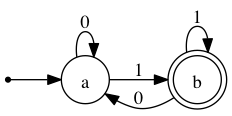
\includegraphics[scale=0.6]{automaatit/nfa.png}
\end{figure}

\begin{figure}[here]
\centering
\caption{Ensimmäisen asteen mutantti $m1$ automaatista $O$, jossa siirtymä tilasta $b$ tilaan $a$ on lisätty aakkosella $1$}
\label{fig:m1}
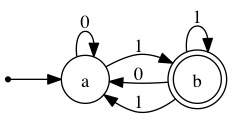
\includegraphics[scale=0.6]{automaatit/m1.png}
\end{figure}

\begin{figure}[here]
\centering
\caption{Ensimmäisen asteen mutantti $m2$ automaatista $O$, jossa siirtymä tilasta $a$ tilaan $b$ korvattu tyhjällä siirtymällä}
\label{fig:m2}
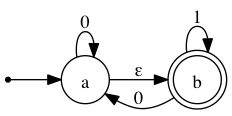
\includegraphics[scale=0.6]{automaatit/m2.png}
\end{figure}

\subsection{Mutaatiot äärellisillä automaateilla}
Äärellisten automaattien tapaukseen mutaatoiden määrittely on helppoa. Olkoon $\Sigma=\{0,1\}$ aakkosto. Voimme nyt määritellä tälle aakkostolle useita eri äärellisiä automaatteja, jotka hyväksyvät vain jotkin tietyt aakkostosta $\Sigma$ koostuvat merkkijonot. Eräs tällainen automaatti löytyy kuvasta~\ref{fig:nfa}, jonka automaatin aloitustila on $a$ ja hyväksyvä tila on $b$. Kyseinen automaatti hyväksyy minkä tahansa merkkijonon, joka loppuu aakkoseen $\sigma = 1$. Määritellään nyt myös joukko mutaatioita $M$. Jokainen mutaatio $m\in M$ on kuvaus, joka korvaa jonkin olemassaolevan tilasiirtymän toisella, poistaa, tai lisää tilasiirtymän. Näitä funktioita kutsutaan mutaatio-operaattoreiksi. Jokainen mutaatio $m$ on siis kuvaus aakkoston $\Sigma$ äärellisten automaattien joukolta itselleen, jossa tämä mutaatio tekee jonkin muutoksen äärelliseen automaattiin. Tarkastellaan joitain kuvan~\ref{fig:nfa} epädeterministisen äärellisen automaatin ensimmäisen asteen mutantteja, eli mutantteja joihin on sovellettu tasan yhtä mutaatio-operaattoria. Korkeamman asteen mutantteja ovat mutantit joihin on sovellettu useampaa kuin yhtä mutaatio-operaattoria.

Kuvat~\ref{fig:m1} ja ~\ref{fig:m2} sisältävät eräät ensimmäisen asteen mutantit alkuperäisestä automaatista. Kuvan~\ref{fig:m1} mutantti eroaa alkuperäisestä automaatista siten, että tilasta $b$ tilaan $a$ on lisätty toinen yhteys. Mutantti kuvassa~\ref{fig:m2} eroaa alkuperäisestä automaatista siten, että yhteys tilasta $a$ tilaan $b$ on vaihdettu tyhjäksi siirtymäksi. Kun tarkastelemme millaisia merkkijonoja nämä mutanttiautomaatit hyväksyvät, huomaamme, että kuvan~\ref{fig:m2} automaatti ei ole ekvivalentti alkuperäisen automaatin~\ref{fig:nfa} kanssa. Automaatit ovat ekvivalentit jos ne hyväksyvät ja hylkäävät täsmälleen samat merkkijonot. Kuvan~\ref{fig:m2} mutantti hyväksyy minkä tahansa merkkijonon annetulla aakkostolla $\Sigma$, sillä tyhjä tilasiirtymä vie hyväksyvään tilaan $b$. Tilasta $b$ voidaan siirtyä nollasiirtymällä tilaan $a$, tai ykkössiirtymällä itseensä. Mikäli siirrytään tilaan $a$, voidaan pysyä tässä tilassa nollasiirtymällä, tai siirtyä hyväksyvään tilaan tyhjällä siirtymällä. Huomataan siis, että alkuperäinen automaatti ei ole ekvivalentti mutantin $m2$ kanssa, eli alkuperäisen automaatin määrittelemä kieli $L(O)$ ei ole sama kuin kuvan~\ref{fig:m2} määrittelemä kieli $L(m2)$.

Kun tarkastellaan kuvan~\ref{fig:m1} mutanttia $m1$, huomataan, että se hyväksyy täsmälleen samat merkkijonot kuin alkuperäinen automaatti $O$, eli $L(O) = L(m1)$. Mutantissa $m1$ on kaikki samat tilasiirtymät kuin automaatissa $O$, joten se hyväkyy vähintään kaikki samat merkkijonot, sillä epädeterminismin johdosta mikä tahansa merkkijono, joka hyväksytään jollakin mahdollisella tilasiirtymäjonolla, hyväksytään. Tämä automaatti ei myöskään hyväksy mitään muita merkkijonoja, sillä lisätty tilasiirtymä ei tuo mitään uusia mahdollisuuksia siirtyä hyväksyvään tilaan $b$, vaan ainoastaan pois siitä. Päästäkseen takaisin tilaan $b$ on taas käytettävä ykkössiirtymää. Tilannetta, jolloin $L(0) = L(m1)$ kutsutaan ekvivalenssiksi. Kaksi automaattia voivat siis olla ekvivalentteja, vaikka ne eivät sisällä täsmälleen samoja tiloja ja tilasiirtymiä.
 
\subsection{Mutaatiot ohjelmointikielissä}
Olkoon $O$ jokin alkuperäinen, jollain ohjelmointikielellä toteutettu ohjelma. Nyt $M$ on joukko mutantteja ja jokainen $m\in M$ on sama ohjelma, mutta siihen on tehty jokin tai joitakin syntaktisia muutoksia. Mutaatoiden luonto riippuu usein käyteystä ympäristöstä. On selvää, että täysin samat mutaatiot eivät käy sekä olio-ohjelmointikieliin, että puhtaasti funktionaalisiin ohjelmointikieliin.

Mutantit tuotetaan ohjelmointikieliin ns. mutaatio-operaattoreilla. Mutaatio-operaattori on funktio, joka tuottaa mutaation annettuun ohjelmaan $O$. Mutaatioiden idea on täysin sama kuin äärellisille automaateille: voidaan korvata, lisätä tai poistaa elementtejä ohjelmakoodista. Käytettävät mutaatio-operaattorit ovat useissa imperatiivisissa ohjelmointikielissä pääosin samat. Agrawal kollegoineen listaavat 76 C-kielen mutaatio-operaattoria~\cite{AgrawalDHHHKMMS89}. Nämä mutaatio-operaattorit pätevät pääosin siis kaikkiin C-pohjaisiin ohjelmointikieliin, kuten Javaan ja PHP:hen, sekä karkeasti muihin imperatiivisiin ohjelmointikieliin. Ne on jaettu seuraaviin ryhmiin: lausemutaatio, operaattorimutaatio, muuttujamutaatio ja vakiomutaatio. Lausemutaatioihin luetaan mm. breakin muuttaminen continue lauseeseen, sekä aaltosulkeiden paikan ja goto lauseen kohteen muuttaminen. Operaattorimutaatioita ovat esimerkiksi aritmeettisten ja loogisten operaattoreiden muuttamiset toisiksi vastaavanlaisiksi operaattoreiksi. Muuttujien mutatointia on mm. viitteiden vaihtaminen toiseksi. Vakioiden mutatointi viittaa vakioiden arvojen päittäin vaihtamiseen, tai yksittäisen vakion arvon manipulointiin. Jokaisesta näistä mutaatiotyypistä on useita variaatioita. Joistakin lähteistä vastaavanlaisia mutaatio-operaattoreita löytyy jopa enemmän.

\subsection{Mutaatiot eri ohjemointiparadigmoissa}
Javassa, sekä muissa olio-ohjelmointikielissä voidaan kokea tarve olio-ohjelmointiominaisuuksiin spesifeille mutaatio-operaattoreille. Kim kollegoineen esittelevät useita olio-ohjelmontispesifejä mutaatio-operaattoreita, esimerkiksi metodien parametrien järjestyksen vaihtaminen, ylikuormituksen poistaminen, metodien ylikirjoitus perinnässä ja monia muita~\cite{KimCM00}. Näiden uusien mutaatio-operaattoreiden lisäksi luokkien sisäistä ohjelmakoodia tulee mutatoida. Mutantteja ei luoda vain pääohjelmasta, vaan jokainen ohjelman yksittäinen komponentti mutatoidaan käytössä olevia mutaatio-operaattoreita käyttäen. Mutaatio-operaattoreita voidaankin lisätä kieli- ja paradigmakohtaisesti melkeinpä loputtomiin. Voidaankin miettiä onko jokainen mahdollinen operaattori tarpeellinen. Osajoukkoa kaikista mahdollisista operaattoreista, jotka tuottavat hyvän kuvan kattavuudesta tilanteessa kuin tilanteessa, sanotaan riittäväksi joukoksi.

Olio-ohjelmointispesifeistä mutaatio-operaattoreista voidaan jo huomata, että paradigman vaihtuessa myös mutaatiotaktiikkaa voidaan joutua muuttamaan. Tämä ei päde ainoastaan olio-ohjelmointiparadigmaan. Mutatoitaessa jotain puhtaasti funktionaalista ohjelmointikieltä, kuten Clojurea voidaan joko mutatoida lähdekoodia, tai mutatoida käännöksen tuottamaa Javan tavukoodia. Tavukoodia mutatoitaessa voidaan käyttää jokseenkin vastaavanlaisia tekniikoita kuin Javalle tarkoitetuilla tavuukodia mutatoivilla mutaatiotestauskehyksillä. Toisaalta voidaan myös mutatoida itse lähdekoodia, jolloin joudutaan keksimään uusia mutaatioita, koska Clojuressa ei ole varsinaiseti operaattoreita, vaan ainoastaan funktioita. Funktioita tulisi korvata toisilla funktioilla, mutta niiden suuri määrä tuottaa ongelmia. Lisäksi Clojure on dynaamisesti tyypitetty kieli, joten sopivien korvaavien funktioiden löytäminenkin ei onnistu helposti esim. paluuarvoja ja argumenttien tyyppejä tarkastelemalla. Clojuresta voidaan myös käyttää Javan luokkia, joten voidaan kokea tarve käyttää myös olio-ohjelmointiparadigmaan liittyviä mutaatio-operaattoreita. Tutkielmassa keskitytään imperatiivisiin ohjelmointikieliin, erityisesti olio-ohjelmointikieliin, kuten Java.

\section{Mutanttien generointi ja käsittely}
Jos käytetään kaikkia mutaatio-operaattoreita, luodaan pienillekkin ohjelmille iso määrä mutantteja. Buddin mukaan generoitujen mutanttien määrä on verrannollinen dataolioiden ja data referenssien määrien tulon kanssa~\cite{Budd}, karkeasti tarkoittaen, että ohjelman koon kasvaessa möys mutanttien määrä kasvaa. Isojen mutanttimäärien tarkastelu on hyvin epätehokasta. Wongin ja hänen kollegoidensa mukaan mutaatiotestauksen laskenta-aika riippuu kahdesta tekijästä: tarkasteltavien testien joukon koosta $|T|$, sekä tarkasteltavien mutanttien määrästä $|M|$~\cite{}. Tämän takia mutanttien generointiin ja käsittelyyn on haettu erinäisiä helpotuksia, jotka voidaan jakaa seuraaviin kategorioihin~\cite{Hussain08}:
\begin{enumerate}
\item Tehdään vähemmän työtä, eli redusoidaan mutanttien määrää
\item Tehdään viisaammin, eli jaetaan laskenta useammalle koneelle ja/tai prosessille
\item Tehdään nopeammin, eli generoidaan mutantit ja suoritetaan sykli nopeammin
\end{enumerate}
Esille tuotuja ensimmäisen kohdan keinoja ovat mm. selektiivinen mutatointi, mutanttien valinta, mutanttien klusterointi eli ryvästäminen, ja korkeamman asteen mutaatiot. Nämä tekniikat pyrkivät redusoimaan käsiteltävien mutanttien määrää. Redusointiongelma voidaan formalisoida seuraavasti: yritetään löytää mutaatioiden $M$ osajoukko $M'$, jolle pätee $K(M) \sim K(M')$, missä $K$ on mutanttien tuottaman kattavuuden laskeva mutaatiokattavuuskuvaus. Mutantteja redusoitaessa pyritään siis löytämään sellainen mutanttien osajoukko, jolla saadaan aikaiseksi mahdollisimman hyvin alkuperäistä joukkoa vastaava mutaatiokattavuus. Tarkoituksena on säästää aikaa, joka kuluu testien suorittamiseen jokaiselle yksittäiselle mutaatiolle. On pidettävä mielessä, että tämän redusointimenetelmän on toimittava ohjelmalle yhtä hyvin myös ohjelman ja testien muuttuessa, sekä yleistyttävä mieluiten kaikille ohjelmille. Seuraavaksi käsitellään mutanttien redusointia, jonka jälkeen esitetään joitain optimointeja syklin nopeuttamiseksi. Useimmat mutaatiotestauskehykset noudattavat jossain määrin kaikkea näitä kolmea nopeutuskeinoa skaalautuakseen suurillekkin ohjelmille. Näihin konkreettisiin toteutuksiin palataan tutkielman lopussa.

\subsection{Selektiivinen mutatointi}
Räjähdysmäistä mutanttien määrää voidaan rajoittaa selektiivisellä mutatoinnilla, missä käyttöön otetaan vain hyvin rajoitettu osajoukko kaikista tarjolla olevista mutaatio-operaattoreista. Nämä mutaatio-operaattorit pyritään valitsemaan niin, että saadaan efektiivisesti mahdollisimman paljon tärkeitä mutaatioita generoitua tällä osajoukolla. Selektiivisellä mutatoinnilla saadaan aikaiseksi paljon vähemmän mutantteja testattavaksi. Jos valituilla mutaatio-operaattoreilla saadaan lähes vastaavia tuloksia, voi tämä olla kannattavaa, sillä mutaatioiden käsittelyyn menevä aika kasvaa räjähdysmäisesti ohjelman koon kasvaessa. 

Oikeiden mutaatio-operaattoreiden valinta on kuitenkin osoittautunut vaikeaksi. Ei voida olla varmoja siitä, että samat operaattorit toimivat hyvin kaikilla eri ohjelmilla. Eräs ratkaisu on valita sellaisia mutaatio-operaattoreita, jotka ovat yksinkertaisia ja joiden on kokeellisesti havaittu tuottavan vastaavia tuloksia suurempien osajoukkojen kanssa~\cite{GrunSZ09}. Tämä on erittäin heuristinen menetelmä, eikä sillä voi odottaa vastaavia tuloksia kohdealueesta ja ohjelman koosta riippumatta. Esimerkkiohjelmien avulla hyväksi todettujen operaattoreiden valinta on kuitenkin nykyisissä mutaatiotestauskehyksissä yleisin tapa ja se perustuu niin sanottuun liitosvaikutukseen: jos annetut testit $T$ havaitsevat kaikki yksinkertaiset virheet ohjelmistossa, ne havaitsevat myös suurimman osan monimutkaisemmista virheistä, jotka ovat koottavissa näistä pienistä virheistä~\cite{DeMilloLS78}. 

Jos valittu mutaatio-operaattoreiden joukko $\mu'$ tuottaa mutantit $M'$ siten, että $K(M) \sim K(M')$, sanotaan että $\mu'$ on riittävä joukko mutaatio-operaattoreita. Mathur esitti $N$-selektiivisen mutatoinnin~\cite{Mathur91}, jolla tarkoitetaan sitä, että $N$ eniten mutaatioita tuottavaa mutaatio-operaattoria jätetään huomiotta mutanttien generoinnissa. Offuttin ja kumppaneiden evaluointi $N$-selektiivisen mutatoinnin tehokkuudesta ja tarkkuudesta osoitti, että kymmenelle FORTRAN ohjelmistolle $2$-selektiivinen mutatointi ei eronnut tilastollisesti tarkkuudeltaan alkuperäisestä mutaatio-operaattorijoukosta~\cite{OffuttRZ93}. Kun $N$:n koko kasvoi entuudestaan, huomattiin, että operaattoreiden hylkääminen yksi kerrallaan vähensi laskenta-aikaa huomattavasti enemmän kuin tarkkuutta. Jos mutaatio-operaattoreiden lähtöjoukko tai annetut ohjelmat olisivat olleet erilaisia, oltaisiin voitu päätyä erilaiseen lopputulokseen. Operaattoreiden eliminoimisessa ei nimittäin otettu huomioon lainkaan niiden tärkeyttä. Tärkeyttä voidaan mitata useilla eri tavoilla, esimerkiksi hyödyllisten ja ekvivalenttien mutanttien suhteella~\footnote{Ohjelmointikielillä ekvivalentit mutantit ovat ohjelmia jotka toimivat täsmälleen samalla tavalla kuin alkuperäinen ohjelma millä tahansa syötteellä. Ekvivalenssia käsitellään tarkemmin kappaleessa 6}. Kun valitaan mutaatio-operaattoreita, halutaan maksimoida tärkeiden mutanttien määrä.

Mutaatio-operaattoreiden $\mu'$ valintaa kaikkien olemassaolevien operaattoreiden joukosta $\mu$ voidaan intuitiivisesti tarkastella myös tilastollisena ongelmana. Olkoon $\mu$ jokin ennaltamääritelty joukko mutaatio-operaattoreita. Osajoukon $\mu'$ löytäminen operaattoreista $\mu$ voidaan nähdä piirteidenvalintaongelmana siten, että jokaista mutaatio-operaattoria esitetään tavalla tai toisella piirteinä tai yksinkertaisimmin vain yhtenä piirteenä. Nyt nämä piirteet muodostavat datamatriisin, josta voidaan löytää ohjaamattoman koneoppimisen menetelmillä tärkeimmät piirteet. Näitä menetelmiä kutsutaan dimensionaalisuuden redusointitekniikoiksi. Tunnetuin näistä on pääkomponenttianalyysi (PCA). Tässä menetelmässä mahdollisesti lineaarisesti toisistaan riippuvaisista piirteistä saadaan transformoitua toinen piirrejoukko, joka on järjestetty varianssinsa perusteella korkeimmasta pienimpään. Näitä piirteitä on lukumäärällisesti vähemmän kuin alkuperäisiä piirteitä. PCA ei kuitenkaan sovellu suoraan mutaatio-operaattoreiden tapauksessa, sillä siitä saadut piirteet eivät enää vastaa alkuperäisiä piirteitä. Koska alkuperäisistä piirteistä halutaan jokin osajoukko, pitää käyttää jotakin menetelmää joka säilyttää piirteet ennallaan, eikä tee niistä koostepiirteitä kuten PCA:ssa. 

Namin ja kumppanit käyttivät kolmea eri menetelmää tähän tarkoitukseen ja arvioivat niiden hyvyyttä mittakaavalla $K(M) \sim K(M')$~\cite{NaminA06}. Mutaatio-operaattorit esitettiin tilastollisesti siten, että jokaiselle mutaatio-operaattorille laskettiin oma operaattorikohtainen mutaatiokattavuus. Näin saatiin 108 piirrettä yhtä monesta mutaatio-operaattorista. Myös kokonaismutaatiokattavuus laskettiin ja tätä pidettiin piirteenä 109. Näiden sarakkeiden arvot täytettiin seitsemän Siemensin C-ohjelman vastaavilla arvoilla. Kaikkien kolmen menetelmän mukaan kaikille seitsemälle ohjelmalle yhteisiä mutaatio-operaattoreita oli melko vähän: menetelmästä riippuen viidestä kymmeneen. Menetelmien välillä ei ollut yhtäkään jokaiselle ohjelmalle ja menetelmälle yhteistä operaattoria. Kuitenkin jokainen menetelmä tuotti yksinään melko hyvän vastaavuuden alkuperäiselle mutaatiokattavuudelle. Paras tulos saavutettiin kaikkien osajoukkojen regressiolla (SUB). Tässä menetelmässä ongelmaa tarkastellaan yksinkertaisena regressio-ongelmana, missä 108:lla ensimmäisellä piirteellä yritetään ennustaa viimeinen. Menetelmällä löydetään jokin tietyn kokoinen osajoukko, joka johtaa parhaaseen mahdolliseen lineaariseen malliin tälle viimeiselle piirteelle. Kohteeksi valittiin tässä kokeessa 20 operaattoria, joka on 19\% alkuperäismäärästä. Muut käytetyt menetelmät olivat agglomeratiiviseen klusterointiin perustuva menetelmä, jossa jokaisesta klusterista valittiin jokin edustava mutaatio-operaattori, sekä eliminaatiopohjainen korrelaatiotekniikka (EBC), jossa jokaisen mutaatio-operaattoriparin välille lasketaan niiden korrelaatio. Tämän jälkeen jokaisesta parista joiden korrelaatio on yli $0.9$ se kumpi tuottaa enemmän mutantteja poistetaan. Jäljelle jäneet mutaatio-operaattorit muodostavat löydetyn osajoukon $\mu'$. Kaikkien osajoukkojen regressio näistä menetelmistä parhaana etsii vain lineaarisia malleja kokonaiskattavuuden kuvaamiseksi. 

Epälineaaristen mallien tarkasteleminen voisi osoittautua hyödylliseksi. Esimerkiksi Gaussilaisten prosessien regressio löytää epälineaarisia regressiomalleja. Myös löydettyjen mallien yleistymistä olisi hyvä tarkastella; miten hyvin tämä joistain ohjelmista opittu malli yleistyy muille ohjelmille: yleistyykö se hyvin saman kohdealueen tai ohjelmointikielen sovelluksille. Lisäksi tässä kokeessa jokaiselle ohjelmalle rakennettiin oma lineaarinen malli, eli käytettiin vain sen ohjelman omaa riviä. Selvä tekijä siihen, miksi ohjelmille ei löydetty yhteisiä mutaatio-operaattoreita, on ohjelmakohtainen ylisovittaminen. Ylisovittamisella viitataan tässä ongelmaan, joka johtuu siitä, että jokaiselle ohjelmalle rakennetaan oma mallinsa. Jos mallin rakentamiseen on käytetty vain yhtä ohjelmaa, se ei todennäköisimmin yleistu ollenkaan muille ohjelmille. Järkevämpää voisi olla rakentaa tämä lineaarinen tai epälineaarinen regressiomalli käyttäen jokaisen ohjelman dataa. Nyt malli yleistyy todennäköisemmin, eikä jokaiselle ohjelmalle tarvitse laskea omaa mallia, vaan riittä mallin laskeminen kertaalleen. Ilman uutta koetta ei voida kuitenkaan sanoa, että tällainen malli tuottaisi enää yhtä hyvää vastaavaa mutaatiokattavuutta. Jokaiselle ohjelmalle oman mallin kouluttaminen on melko raskas prosessi ja tätä tulee välttää. Lisäksi jos mallin yleistymisestä ei ole takeita edes samankaltaisille tai saman kohdealueen tai alustan sovelluksille, joudutaan malli laskemaan uudestaan aina ohjelman muuttuessa. Tämä on selvä riski, sillä selektiivisen mutaation päätarkoitus on useimmiten nimenomaan laskenta-ajan vähentäminen.
% Tässä vois keskustella tarkemmin jotain spesifejä tapoja mitä on käytetty, kts. variable_reduction paperi (done) ja sen ylempi lähdelistasta (tarpeellista? siellä vaan CBLARS)

\subsection{Mutanttien valinta}
Toinen keino on vähentää tarkasteltujen mutanttien määrää on vähentää suoraan käsiteltäviä mutantteja. Mutanttien valinnassa generoiduista mutanteista $M$ valitaan pienempi osajoukko $M'$, joka sisältää vain ennalta sovitun määrän alkuperäisistä mutanteista. Valinta voidaan tehdä esimerkiksi satunnaisesti, jossa on ongelmansta. Satunnaisesti valitut mutantit eivät anna kovinkaan hyviä takeita siitä, että $K(M) \sim K(M')$. 

Hussain esitteli tutkielmassaan mutanttien klusteroinnin~\cite{Hussain08}. Tämä tekniikka perustuu ohjaamattoman koneoppimisen tekniikkaan, ryvästämiseen (klusterointiin), jossa tarkoituksena on löytää leimaamattomasta datasta samankaltaisia ryppäitä. Pohjimmiltaan tarkoitus on sama kuin mutanttien valinnassa. Mutanttien klusteroinnissakin mutanttien kokonaisjoukosta $M$ valitaan joukko mutaatiota $M'$. Osajoukko $M'$ muodostuu näistä valituista mutanteista. Näin valitaan vain osa toisiaan muistuttavista mutanteista, jolloin saadaan varmemmin joukko $M'$, jolle pätee $K(M) \sim K(M')$. 

Tutkielmassaan Hussain esittää ohjelman jokaista mutanttia omana dataolionaan, eli klusteroinnille tyypillisesti muodostetussa datamatriisissa jokaiselle mutantille on oma rivinsä. Jokaisen mutantin piirteet koostuvat binäärisestä $n$ pituisesta rivivektorista, missä $n$ on annettujen testien lukumäärä $|T|$. Vektorin indeksissä $i$ arvo $v(i) = 1$, jos testi $T_i$ tappaa tätä riviä edustavan mutantin. Muuten $v(i) = 0$. Klusteroinnissa mutantit jaetaan ryhmiin sen mukaan, mitkä testit ovat niille kuolettavia. Jokaisesta tällaisesta klusterista $C_{i}$ valitaan sitten vain jokin osajoukko mutantteja tai jopa vain yksi tämän klusterin edustajaksi. 

Kokeessaan Hussain käytti partitionaalista K-means-algoritmia, sekä hierarkista agglomeratiivista klusterointia. Klusterointialgoritmit eivät kuitenkaan ole täysin stabiileja ja ovat potentiaalisesti hitaita suorittaa, kun $|M|$ on suuri. K-means-algoritmi on hyvin sensitiivinen klustereiden alkuarvojen asettamiselle, ei taatusti konvergoidu globaaliin optimiin, ja tuottaa mallinvalintaongelmia: klustereiden määrä $k$ pitää antaa algoritmille parametrina. Se tulee siis löytää jotenkin ennen algoritmin suoritusta. Agglomeratiivinen klusterointi taas vaatii pitkälti silmämääräistä tarkastelua ja voi vaatia ylimääräisiä ohjelmistokehittäjien työtunteja, jos klusterointia suoritetaan useasti. Mutanttien klusterointi taatusti hidastaa mutaatiotestauksen automatisoitua osaa, eli testien suorittamista mutanteille ja mutanttien generointia, sillä siinä mutanttien valinnan onnistumiseksi jokaiselle mutantille on suoritettava kaikki testit joukossa $T$. Lisäksi on hieman ongelmallista, että eri mutantit saatetaan jaotella ryhmiin eri tavoin jokaisella klusteroinnin suorituskerralla K-means-algoritmin epästabiiliuden vuoksi. Se voi kuitenkin tehokkaasti vähentää niiden mutanttien määrää, joita ohjelmoijien pitää tarkastella joka on omanlaisensa etu. Ne testit, jotka tappavat näitä valittuja mutantteja ovat ohjelman kannalta tärkeät testit, olettaen $K(M) \sim K(M')$. Testit jotka eivät tapa yhtäkään mutanttia ovat todennäköisesti turhia, ja ne voidaan poistaa testaussyklistä.

\subsection{Korkeamman asteen mutaatiot}
Korkeamman asteen mutaatioiden perus ajatus on käyttää mutantteja, jotka koostuvat useammasta vaikeammin tapettavasta ensimmäisen asteen mutantista. Korkeamman asteen mutantit ovat mutantteja, joihin on sovellettu useampaa mutaatio-operaattoria. Jokainen korkeamman asteen mutantti on jaoteltavissa niihin ensimmäisen asteen mutantteihin, joihin jokaista tämän mutantin yksittäistä mutaatio-operaattoria on sovellettu. Vaikeammin tapettavia korkeamman asteen mutantteja käytettäessä halutaan saada aikaan uusi mutanttijoukko $M'$, jolle pätee $|M| > |M'|$. Sopivien mutanttien löytäminen tähän tarkoitukseen on kuitenkin hankalaa. 

Jia ja Harman esittelivät korkeamman asteen mutanttien konseptin, sekä vahvasti liitetyt korkeamman asteen mutantit~\cite{JiaH08b}. Vahvasti liitetyille korkeamman asteen mutanteille $m^h$ pätee seuraava ehto: jos mutantti $m^h$ tulee tapetuksi, myös jokainen ensimmäisen asteen mutantti $m^1_i$ tulee tapetuksi. Ensimmäisellä tarkastelulla korkeamman asteen mutantteja voidaan generoida vielä enemmän kuin ensimmäisen asteen mutantteja. Jos oletetaan, että ensimmäisen asteen mutantteja on $n$ kappaletta, on näistä mahdollista generoida $n^n$ korkeamman asteen mutanttia. Kuitenkin kun korkeamman asteen mutantteja käytetään tarkasteltavien tapausten minimointiin, halutaan hakea nimenomaan vahvasti liitettyjä korkeamman asteen mutantteja, joita on määrällisesti vähemmän kuin itse ensimmäisen asteen mutantteja joista ne koostuvat. 

Jia ja Harman etsivät korkeamman asteen mutantteja kolmella eri lähestymistavalla: ahne algoritmi, geneettinen algoritmi, ja kukkulalle kiipeämisalgoritmi. Näitä algoritmeja varten määriteltiin korkeamman asteen mutanteille hyvyysfunktio $f = \frac{\text{fragiliteetti}({m^h})}{\text{fragiliteetti}({m^1_1, ..., m^1_n})}$, missä $\text{fragiliteetti}(m_i, ..., m_n) = \frac{|\bigcup{i=1}^{n} \text{tappaa}(m_i)|}{|T|}$. Funktio $\text{tappaa}$ palauttaa ne testit jotka tappavat sille annetut mutantit. Mutanttijoukon fragiliteetti on siis niiden testien määrän summa, jotka tappavat sille annetut mutantit jaettuna kaikkien testien lukumäärä. Kun fragiliteetti lähenee yhtä, on mutantti heikko. Kun fragiliteetti lähenee nollaa mutantti on vahva. Jos arvo on täsmälleen nolla, on mutantti selvinnyt ja se on potentiaalisesti ekvivalentti. Fitnessi eli hyvyys on määritelty fragiliteetin avulla siten, että mutantin fitnessi on sen fragiliteetin suhde sen ensimmäisen asteen komponenttimutanttien fragiliteettiin. Kaikki kolme optimointialgoritmia käyttävät tätä fitnessiä. 

Geneettinen algoritmi osoittautui tehokkaimmaksi tavaksi löytää halutunlaisia korkeamman asteen mutantteja, mutta kahta muuta esiteltyä algoritmia voidaan käyttää tämän lisäksi tulosten parantamiseksi. Kuuden ohjelman tutkimuksessa selvitettiin vain näiden mutanttien löytymiseen ja määrään liittyviä seikkoja. Mutanttien määrä väheni erittäin tehokkaasti. Miten paljon tämä lähestymistapa nopeuttaa mutaatioanalyysiä, jäi tarkastelematta. Varsinkin geneettinen algoritmi voi potentiaalisesti viedä hyvin paljon aikaa, jos halutaan löytää läheskään optimaalisia mutantteja. Sen käyttäminen voi siksi viedä paljon lisää aikaa mutanttien generointivaiheessa. Jos tämä vähentää tehokkaasti ekvivalenttien mutanttien määrää voi se säästää koko mutaatioanalyysiprosessin aikaa. Kirjoittajat eivät myöskään tarkastelleet heidän generoimiensa mutanttien vastaavuuttaa alkuperäisiin mutantteihin. On tärkeää tietää miten hyvin korkeamman asteiden mutanttien mutaatiokattavuus vastaa alkuperäistä kattavuutta ennen menetelmän käyttöönottoa.

\subsection{Mutanttianalyysin optimointi}
Myös yksittäisen mutanttien testausprosessia voidaan optimoida. Ensimmäinen luonnollinen optimointi on ajaa testit yksittäisiä mutantteja vasten rinnakkain. Toinen tekninen optimointi on ajaa vain tarvittavat testit jonkin mutantin tappamiseksi. Rivi- ja haarakattavuutta tarkastelemalla voidaan selvittää mitkä testit suorittavat mutaatiokohdan ohjelmassa, ja valita vain ne tarkasteltavaksi. Jos jokin testi testaa täysin mutaatiosta riippumatonta osaa koodissa, voidaan se jättää suorittamatta. Tämä optimointi on käytössä mm. Javalanche mutaatiotestauskehyksessä~\cite{SchulerZ09}.

Mutanttien analysointi vie paljon aikaa erityisesti käännettävissä ohjelmointikielissä. Jokainen yksittäinen mutantti $m\in M$ pitää kääntää kun testit ajetaan tälle mutantille. Tämä ongelma voidaan helposti välttää tulkattavissa ohjelmointikielissä, kuten Rubyssa ja Pythonissa, jotka ovat moderneja, paljon käytettyjä skriptauskieliä. Tulkattavissa kielissä voidaan ajaa ohjelmakoodi sellaisenaan, pitäen mielessä mutaatiokohta. Kun saavutaan mutatoidulle riville, se suoritetaan sen mutatoidulla versiolla. Näin muistissa tarvitsee pitää vain mutatoitu rivi ja suoritus tapahtuu vain alkuperäistä ohjelmaa tulkkaamalla. Joissain mutaatiotestauskehyksissä ollaan simuloitu tätä käyttäytymistä käännettäville ohjelmointikielille. 

Javalanche~\cite{SchulerZ09} on Java ohjelmille toteutettu mutaatiotestauskehys, joka mutatoi suoraan Javan tavukoodia. Tällä vältytään jokaisen mutantin yksittäisellä kääntämiseltä ja päästään samaan vaikutukseen kuin tulkatuilla ohjelmointikielillä. Tavukoodin hyödyntämisen mutatoinnissa esittelivät ensimmäisen kerran Ma ja kumppanit~\cite{MaOK05}. Aikaisemmin kääntämiseen kuluvan ajan vähentämiseksi tutkittiin ns. supermutanttien generointia~\cite{}, jossa alkuperäisestä ohjelmasta $O$ luodaan vain yksi mutantti, joka esittää kaikkia yksittäisiä mutantteja $m\in M$. Supermutantin kääntämällä joudutaan kääntämään vain yksi ohjelma. Supermutantti on kuitenkin kooltaan suurempi ja sen käsittelyn toteuttaminen hankalaa. Tavukoodin mutatointi suoraan on paljon yksinkertaisempi ja vähintään yhtä tehokas vaihtoehto. Tavukoodin mutatointikaan ei ole helppoa tai mahdollista kaikissa tapauksissa, joten näissä tapauksissa supermutanttien käyttäminen voi olla houkutteleva vaihtoehto.

\section{Ekvivalentit mutantit}
Ekvivalentit mutantit ovat alkuperäisen ohjelman mutantteja, jotka ovat toiminnallisuudeltaan kuitenkin täysin vastaavia alkuperäisen ohjelman kanssa, aivan kuten äärellisten automaattien tapauksessa. Niiden läsnäolo johtaa siihen, ettei mutaatiokattavuus ole numeerisesti 100\%, vaikka todellisuudessa testit kattavat kaikki epäekvivalentit mutantit. Ekvivalenttien mutanttien tunnistaminen manuaalisesti on rasittavaa ja aikaavievää~\cite{GrunSZ09}. Schuler ja kumppanit selvittivät kokeellisesti, että satunnaisesti generoitujen mutanttien ekvivalenssin tunnistaminen kestää noin 15 minuuttia yhtä mutanttia kohden melko laajoissa ohjelmistoissa. Tappamattomista mutanteista noin 45\% havaittiin ekvivalenteiksi. Tämä prosentuaalinen osuus kasvaa entisestään testijoukon $T$ kattavuuden parantuessa edelleen~\cite{SchulerZ10}. Lisäksi on kokeellisesti huomattu, että jos ekvivalenssia ei tutkita tarkkaan, voidaan tehdä virheitä ja leimata joitain tapettavia mutantteja ekvivalenteiksi. Huolimaton selviytyneiden mutanttien tarkastelu voi siis antaa myös päinvastaiseen suuntaan virheellisen kuvan testien kattavuudesta, ja pahimmillaan johtaa liialliseen luottamukseen ohjelman toimivuudesta. Formaalimmin ekvivalenssi voidaan määritellä siten, että jos alkuperäinen ohjelma ajatellaan funktiona $O$ ja mutantti funktiona $m$ niiden tulosteet ovat samat kaikille syötteille $s$, eli $\forall s(O(s) = m(s))$. Ei siis ole olemassa testiä $t_i \in T$, joka erottaa mutantin $m$ alkuperäisestä ohjelmasta $O$.
% Eti Acree: On mutation, sanotaan et 80% ekvivalenteista tunnistetaan oikein

Ekvivalenttien mutanttien tunnistaminen automaattisesti on hankalaa. Voidaan jopa osoittaa, että kahden ohjelman ekvivalenssin tarkistaminen on ratkeamaton ongelma~\cite{}. Alhaisten asteitten mutantit ovat kuitenkin erikoistapauksia tästä ongelmasta, sillä tällöin mutantti poikkea alkuperäisestä ohjelmasta hyvin pienissä määrin, ja vain syntaktisesti. Tutkielmassa esitetään seuraavaksi menetelmiä joista huomataan, että joissain tapauksissa ekvivalenssi voidaan päätellä algoritmisesti ja muissa tapauksissa voidaan käyttää erilaisia tekniikoita ekvivalenssin estimoimiseen tai arvaamiseen. Ekvivalenssia ei välttämättä tarvitse suoraan yrittää ennustaa, vaan selviytyneet mutantit voidaan vaikkapa järjestää niiden ekvivalenssin todennäköisyyden mukaan pienimmästä suurimpaan, jolloin ohjelmoijilla on jonkinlainen käsitys siitä, kuinka tarkkaan kutakin mutanttia tulee tarkastella.


\subsection{Kääntäjän hyödyntäminen}
Ekvivalentteja mutantteja voidaan myös vähentää tunnistamalla niitä mitä voidaan täysin varmasti päätellä. Eräs tapa on käyttää hyväksi käännettävien ohjelmointikielten kääntäjää. Kääntäjät suorittavat useita optimointeja käännettävälle koodille. Kun jokin mutaatio täyttää jonkin optimointisäännön tai tuottaa käänteisen optimoinnin ohjelmaan, voidaan voidaan suoraan täydellä varmuudella todeta mutantin ekvivalenssi. Kääntäjää hyödyntämällä voidaan kuitenkin tunnistaa vain hyvin rajattu osa kaikista ekvivalenteista mutanteista. Lisäksi moni nykyään käytetyistä ohjelmointikielistä on tulkattava, vähentäen tämän menetelmän hyödyllisyyttä ohjelmointikielten yleisessä tapauksessa.

\subsection{Rajoituspohjainen testaus}
Rajoituspohjaisen testauksen alkuperäinen idea on löytää ohjelman syöteavaruudelle mahdolliset rajoitukset ja käyttää näitä tietoja testisyötteen generoimiseksi. Näitä rajoituksia ovat syötteelle $x \in \mathbb{Z}$ esimerkiksi $x > 5$ ja $x <= 2$. Tätä tekniikkaa voidaan soveltaa ekvivalenssin tunnistamiseen~\cite{OffuttP96}. Jotta testi voi tunnistaa mutantin, ohjelmalta vaaditaan tiettyjä ominaisuuksia. Ensinnäkin mutatoitu lause pitää olla saavutettavissa. Jos näin ei ole, ei mikään testi voi mitenkään tappaa mutanttia. Toisekseen jokin ohjelman suorituksen tilan tulee olla eri kuin mutatoimattomassa ohjelmassa mutatoidun lauseen suorituksen jälkeen. Muuten molemmat ohjelmat tuottaisivat välttämättä saman lopputuloksen, eikä testi voisi mitenkään tappaa mutanttia. Kolmannekseen mutanttiohjelman lopputilan tulee erota alkuperäisen ohjelman viimeisestä tilasta. Muuten näiden ohjelmien lopputulos olisi sama. Kaikki näistä kolmesta ehdosta on pädettävä jollakin syöteavaruuden alkiolla $s \in S$, tai muuten mutantti on ekvivalentti. 

Offutt ja kumppanit kehittivät Equivalencer nimisen työkalun, joka etsii ristiriitoja tunnistaen näitä ehtoja. He onnistuivat tunnistamaan seitsemästä laajemmasta ohjelmasta 60\% ekvivalenteista mutanteista. Pienille ohjelmille menetelmän huomattiin toimivan huonommin johtaen kaikkiaan 11:lle käytetylle ohjelmalle keskimäärin 45\% tunnistettuun mutanttiin kaikista ekvivalenteista mutanteista. Heidän menetelmänsä hidasti testien suoritusta merkittävästi, mutta ekvivalenttien mutanttien käsin tunnistamiseen kuluva aika on potentiaalisesti paljon suurempi, joten ainakin sopusuhtaisen kokoisille ohjelmille tämän tekniikan käyttö vaikuttaa järkevältä. Tekniikkaa ei kuitenkaan ole testattu isoilla ohjelmilla, joten ei ole varmaa miten nopeasti sen tuoma lisäys suoritusaikaan alkaa kasvamaan liian suureksi, tai miten suuri osa ekvivalenteista mutanteista löytyy realistisilla tuotantokäytössä olevilla ohjelmistoilla. Rajoituksia ei tarvitse etsiä kuin niille mutaatioille jotka selviävät, joten sen aiheuttama lisäys suoritusaikaan riippuu annetun testijoukon kattavuudesta ja käytetyistä mutaatio-operaattoreista.

\subsection{Selviytyneiden mutanttien järjestäminen}
Zeller ja kumppanit ovat tutkineet, miten ekvivalentit mutantit vaikuttavat ohjelman suoritukseen verrattuna tapettaviin mutantteihin. Käyttäen apuna jotakin mittaa mutantin vaikutuksesta eli impaktista ohjelman suoritukseen, he pyrkivät saamaan jossain määrin mutantin epäekvivalenssin todennäköisyyden kanssa korreloivan arvon. Näitä mittoja ollaan hyödynnetty Javalanchessa listaamaan selviytyneet mutantit jonkin prioriteetin mukaan. Ne mutantit, joilla tämä mitta on korkea, ovat todennäköisemmin tapettavissa, kuin ne joilla se on matala. Tämä mitta voi olla hyödyllinen ohjelmoijalle, joka yrittää päätellä selvinneiden mutanttien ekvivalenssia. Mahdollisena mittana ollaan tutkittu vaikutusta lausekattavuuteen~\cite{GrunSZ09}~\cite{SchulerZ10}, sekä ohjelmasta pääteltyjen invarianttien rikkomuksia~\cite{SchulerDZ09}.

Javalla kirjoitetulla esimerkkiohjelmistolla tutkittiin alustavasti, miten mutaatioiden tuottamat muutokset koodikattavuuteen korreloivat tapettavuuden kanssa~\cite{GrunSZ09}. Huomattiin, että suurin osa niistä mutanteista jotka vaikuttavat eniten koodikattavuuteen, eivät ole ekvivalentteja. Vastaavasti iso osa niistä mutanteista jotka vaikuttavat kattavuuteen vähiten ovat ekvivalentteja. Mutanttien listaaminen tämän järjestelyn perusteella vaikutti siis alustavasti hyödylliseltä. Tutkimukesssa käytettiin vain yhtä ohjelmistoa, joten mitään isoja johtopäätöksiä on vaikea vetää. Tulosten innostamana Schuler ja kumppanit tekivät jatkotutkimuksen, jossa mutantin vaikutusta ohjelman lausekattavuuteen, sekä kaikkien ohjelman metodien paluuarvoihin, tarkasteltiin. Paluuarvot tallennettin kokonaislukuihin siten, että yhtä paluuarvoa esitettiin sen toString() kutsusta tehtynä kokonaislukutiivisteenä tilan siistämiseksi, sillä suurissa ohjelmissa on niin monia metodikutsuja, että jokaisen eksplisiittisen paluuarvon tallentaminen vie liikaa tilaa ja käyttää paljon aikaa levylle kirjoittamiseen. Seitsemästä ohjelmasta valittiin 20 mutanttia tarkasteltavaksi. Tarkasteltavista ohjelmista niiden mutanttien keskuudessa, joilla on suurin vaikutus kattavuuteen tai paluuarvoihin enintään 10\% oli ekvivalentteja. Kattavuuden ja paluuarvojen vaihtelun tarkastelu havaittiin hyödylliseksi ekvivalenssin estimoinnissa.

Mikäli tätä informaatiota halutaan hyödyntää suoraan ekvivalenssin tunnistamiseen, voidaan mutantit luokitella esimerkiksi ekvivalenteiksi ja epäekvivalenteiksi. Jos päätetään jokin kynnysarvo $t$, voidaan sanoa, että mutantti on epäekvivalentti jos ja vain jos sen impakti $i$, eli sen tuoma muutos rivikattavuuteen ja ohjelman paluuarvoihin $i > t$. Muut mutantit luokitellaan ekvivalenteiksi. Kannattavampaa voi olla luokitella hyvin korkealla arvolla $t$ hyvin todennäköisesti epäekvivalentit mutantit, ja jättää muut mutantit luokittelematta. Näin ohjelmoijan ei tarvitse välittää lainkaan niistä mutanteista, joilla epäekvivalenssin todennäköisyys on hyvin suuri. Zellerin ja kumppaneiden jälkimmäinen seitsemän ohjelman tutkimus antaa jo paljon uskottavamman kuvan tämän impaktimetriikan hyvyydestä, kuin aikasempi yhden Java-ohjelman tutkimus. Ei voida kuitenkaan täysin varmasti väittää tulosten yleistyvän kaikille ohjelmille tai edes kaikille Java-ohjelmille. Datasta valitut ekvivalentit ja epäekvivalentit mutantit eivät anna täysin holistista kuvaa kaikista mutanteista, sillä jokaisesta ohjelmasta valittiin selvinneistä mutanteista vain osajoukko tarkasteltavaksi.

Invarianttirikkomusten ja ekvivalenssin korrelaation tarkastelemiseksi Javalanche-mutaatiotestauskehykseen liitettiin komponentti, joka luo lähdekoodista syötetiedostoja DAIKON:ille~\cite{ErnstPGMPTX2007}. DAIKON on ohjelmisto, jonka tarkoituksena on löytää dynaamisesti invariantteja sille annetusta syöteohjelmasta. Se tarkkailee ohjelman suoritusta ja kirjaa ylös eri ohjelman tiloissa päteneitä ehtoja. Näitä invariantteja voidaan päätellä testejä suoritettaessa. Generoiduista mutaatioista voidaan selvittää niiden rikkomien invarianttien määrä, ja pitää tätä mittana mutantin vaikutuksesta ohjelman toimintaan. Tilastollisen analyysin pohjalta Schuler ja kumppanit totesivat invariantteja rikkovien mutanttien olevan kaksi kertaa todennäköisemmin tapettavissa. Havaittiin seuraavaa: eniten invariantteja rikkovat mutantit ovat todennäköisemmin epäekvivalentteja, kuin vähiten invariantteja rikkovat. Invariantteja rikkovat mutantit ovat kuitenkin harvinaisia: vain noin 19\% epäekvivalenteista mutanteista rikkovat todennäköisesti invariantteja, joten invarianttien käyttäminen yksin mutaatioiden impaktin mittana ei ole järkevää. Invarianttien tarkastelu voi kuitenkin olla hyödyllistä yhdistää esimerkiksi edellä esiteltyyn kattavuusanalyysiin.

\section{Mutaatiotestaus käytännössä: PIT}
PIT on on Java-kielelle kehitetty mutaatiotestauskehys, joka saadaan integroitua paljon käytettyihin Javan projektinhallintatyökaluihin, kuten Maveniin. PIT on JUnit-kehyksen päälle rakennettu mutaatiotestikehys, joka tarjoaa automaattisen mutaatioiden generoinnin Java-projekteihin mutatoimalla Javan tavukoodia, välttäen tarpeen kääntää jokainen mutantti erikseen. PIT tunnistaa mutatoitavat luokat ja ohjelman pakkausrakenteesta löytyvät testit automaattisesti. Mutaatiotestaussyklin tuloksena on mutaatiokattavuusraportti, josta löytyy kiinteän kattavuusprosentin lisäksi jokaisen mutantin mutaatiokohta, mutaatiotyyppi, sekä tieto siitä, onko mutantti tapettu vai ei. Nämä raportit ovat mutanttikohtaisia. Mutantit leimataan niiden tarkastelun jälkeen johonkin kuudesta eri luokasta: tapettu, selviytynyt, virheellinen tavukoodiltaan, aikakatkaistu, muistivirheellinen tai suoritusvirheellinen. Virheellisellä tavukoodilla viitataan käännösvirheeseen. Aikakatkaistu mutantti taas usein viittaa loputtomaan silmukkaan ohjelmassa. Muistivirhe ja suoritusvirhe viittaavat ajon aikana mahdollisiin Javan virtuaalikoneen tuottamiin virheisiin, jotka aiheuttavat poikkeuksen. Mutantti voi olla sellainen, että se johtaa virtuaalikoneen muistin ylikuormittamiseen, tai aiheuttaa virheitä koodin suorituksessa. Nämä mutantit voidaan siten jättää huomioimatta, eikä niitä leimata virheellisesti selviytyneiksi.PIT suorittaa jokaiselle mutantille vain tarpeelliset testit Javalanchen tapaan, tarkastellen testien rivikattavuutta säästääkseen resursseja.

PITin mutatointi tapahtuu sen mutaattorien avulla. Mutaattorit ovat luokkia, jotka soveltavat joitain hyvin samankaltaisia mutaatio-operaattoreita. Mutaattoreita on 13 kappaletta, joista kolme on vasta kokeiluvaiheessa. Konditionaalisen rajan mutaattori esimerkiksi vaihtaa $<$ operaattorit $<=$ operaattoreiksi, sekä toisin päin, ja tekee saman myös epäyhtälön toiseen suuntaan. Kontionaalisen rajan negatointimutaattori vaihtaa kaikki loogiset operaattorit niiden negaatioiksi, esim. $==$ mutatoidaan $!=$, sekä $<$ mutatoidaan $>=$. Matematiikkamutaattori mutatoi minkä tahansa kokonais- tai liukulukujen aritmeettisen operaattorin toiseksi. Esimerkiksi $+$ operaattorista tulee $-$, $\&$ operaattorista tulee $|$ ja $\%$ operaattorista tulee $*$. Tarkempi lista näistä operaattoreista löytyy matematiikkamutaattorin operaattorilistauksesta~\cite{PITMathMutations}. Kasvatusmutaattori vaihtaa muuttujan inkrementoinnit dekrementoinneiksi ja toisin päin. Paluuarvottomien metodikutsujen mutaattori poistaa metodikutsut, joilla ei ole paluuarvoa. Paluuarvollisten metodikutsujen mutaattori korvaa jonkin metodin paluuarvon sen paluuarvon tyypin oletusarvolla. Kontruktorimutaattori korvaa kontruktorikutsut null-arvolla. Tässä listattiin vain ne mutaattorit jotka eivät ole kokeiluvaiheessa.

PIT-kehyksen kymmenestä epäeksperimentaalisesta mutaattorista seitsemän ovat oletukselta käytössä. Näistä mutaattoreista saatava mutaatio-operaattoreiden määrä ei ole yhtä laaja kuin aiemmin raportoidut kattavat luettelot olemassaolevista operaattoreista. PITin operaattorit on valittu siten, että ne ovat lähellä tyypillisiä ohjelmoijien virheitä, sekä mahdollisimman stabiileja. Stabiiliudella tässä yhteydessä tarkoitetaan mutaatio-operaattorin tuottavan mahdollisimman vähän ekvivalentteja mutantteja suhteessa ekvivalentteihin mutantteihin. PITin vahvuus on juuri tämä operaattorien valinta. Niiden vähyys takaa sen, että mutaatioanalyysi sujuu tarpeeksi nopeasti skaalautuakseen myös laajemille ohjelmistoille. Lisäksi stabiilit mutaatio-operaattorit takaavat ekvivalenttien mutanttien vähäisen määrän.

PIT tarjoaa myös viisi suoritusaikaoptimointia, jotka voidaan kytkeä päälle haluttaessa. Nämä optimoinnit ovat:
\begin{enumerate}
	\item Jos luokka, jossa oli viime testisyklillä loputon silmukka, ei ole muuttunut, todetaan, että siinä on edelleen silmukka.
	\item Jos mutaatio tapettiin edellisessä syklissä, eivätkä mutatoitu luokka tai mutantin tappanut testi ole muuttuneet, todetaan, että mutantti kuolee uudellakin syklillä.
	\item Jos mutantti selvisi edellisellä syklillä eikä sen testien kattavuuden alueella ole muutoksia, todetaan sen selviävän uudestaan. 
	\item Jos mutantti on tapettu edellisellä kierroksella ja sen tappanut testi on muuttunut, nostetaan tämä mutantti tärkeimmän prioriteetin mutantiksi.
	\item Jos jollain luokalla on useita selviytyneitä mutantteja viime syklissä, voidaan nämä mutaatiot ottaa käyttöön samanaikaisesti ja ajaa testit tällä niinsanotulla metamutantilla. Mikäli tämä metamutantti ei kuole, pitää mutaatiot analysoida yksitellen. Jos taas tämä metamutantti tapetaan, säästetään suoritusaikaa ja todetaan, että kaikki kyseiset mutantit tapettaisiin myös yksitellen.
\end{enumerate}
Nämä optimoinnit kytkettyinä tehostavat PITin suorituskykyä ja skaalautuvuutta edelleen. Niitä ei kuitenkaan ole täysin viisasta käyttää, sillä neljättä optimointia lukuunottamatta ne voivat aiheuttaa virheellisen analyysin. Javassa luokkien käyttäytyminen ei riipu pelkästään sen omasta koodista, vaan myös sen riippuvuuksista muihin luokkiin. Vaikka luokka itse ei olisi muuttunut, sen käyttäytyminen ei välttämättä pysy samana jos esimerkiksi jokin luokka, josta se on riippuvainen, on muuttunut. PIT ei havaitse muita muutoksia luokkaan kuin luokan itsensä, sekä sen perimien yliluokkien muutokset tavukoodista. Näitä optimointeja voidaan ottaa käyttöön luottamalla oletukseen, että luokkien käyttäytyminen muuttuu harvoin ilman, että sen oma lähdekoodi muuttuu. Viimeinen esitelty optimointi lisäksi tuo ylimääräisen riskin: mutantit voivat olla päällekkäisiä, jolloin ylikirjoittavan mutantin tappaminen ei välttämättä implikoi ylikirjoitetun mutantin tappamista.
% jotain kuvia raporteista
\begin{figure}[here]
\centering
\caption{PITest mutaatiotestauskehyksen tuottamat mutantit raportoituna suorituksen jälkeen}
\label{fig:mutantit}
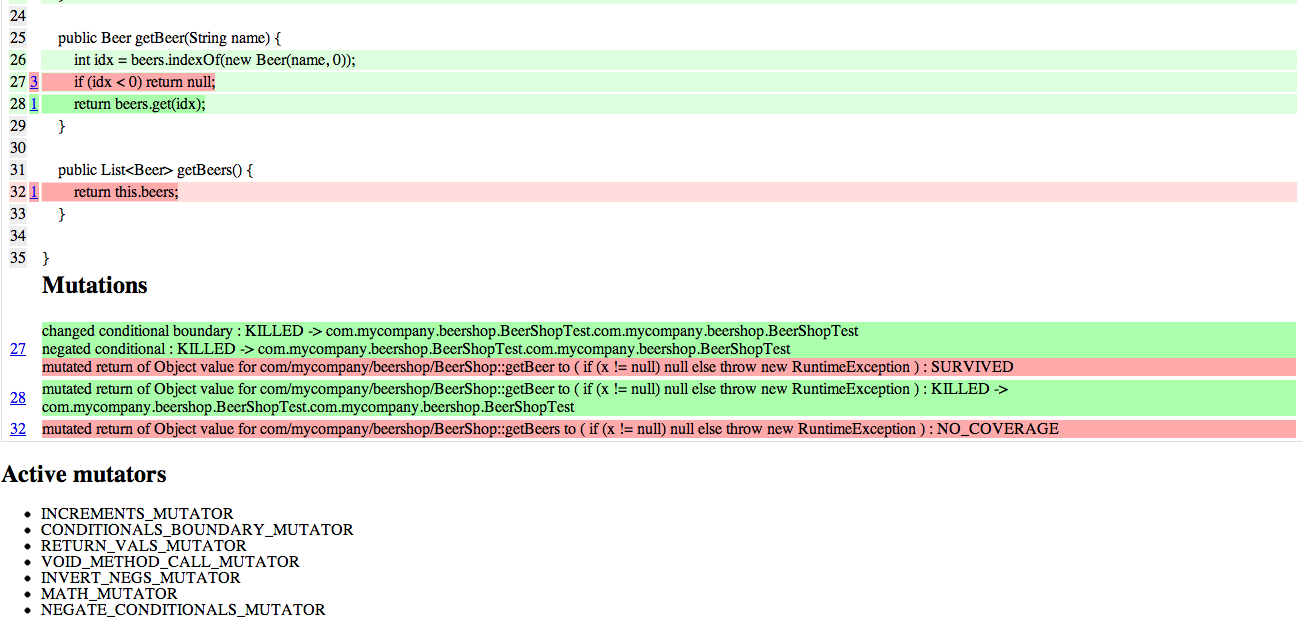
\includegraphics[scale=0.4]{freimarikuvat/mutantit.png}
\end{figure}

\section{Testaus käytännössä}
Cobertura ja sitä syrjäyttävä JaCoCo ovat käytetyimmät testauskattavuustyökalut Java-ympäristössä. Ne tarjoavat samantapaisen HTML muotoisen testikattavuusraportin kuin PIT. Tämä raportti kuitenkin sisältää vain raportin rivi- sekä haarakattavuudesta. Cobertura näyttää rivikattavuuden ja haarakattavuuden vierekkäisinä värityksinä jokaisella rivillä. Jos jollain rivillä on punaista, jomman kumman kattavuusmetriikan mukaan testeissä on puutteita. Kuitenkin kuten aiemmin todettiin, nämä kattavuusmetriikat eivät kuvaa testien ideaalista kattavuutta kovinkaan hyvin. Raportista on kuitenkin helppo huomata jos kokonaisia osia koodista on jäänyt testeissä huomiotta ja mitkä nämä osat ovat. Edellisen kappaleen PITin raporteista huomataan, että yksi mutantti selvisi hengissä, koska testit eivät kattaneet sitä sitä. On siis järkevää käyttää myös Coberturan ja JaCoCon kaltaisia perinteisempiä testikattavuustyökaluja rivi- ja haarakattavuuden selvittämiseksi. Kun nämä kattavuudet ovat 100\%, voidaan siirtyä mutaatiokattavuuteen. Cobertura ja vastaavat työkalut ovat tehokkaampia löytämään niitä koodinpätkiä, mitä ei kateta testeillä. Siksi on järkevää ensin varmistaa, että testit tosiaan suorittavat ohjelmasta halutut osat ennen paljon hitaampaa mutaatiotestausta. Mutaatiotestaus on erittäin hyödyllinen testaajan työkalu. Silti useimmissa ohjelmistotuotantoprojekteissa se ei ole käytössä. Heuristisia mutaatiotestauskehyksiä, kuten PIT, tulisi käyttää enemmän. 
% Tää pitäs kyl siirtää, ja onks tää ees järkevä?
% Tän vois ehkä oikeestaan mergee yhteenvetoon

\section{Yhteenveto}
Mutaatiotestaus on testausmenetelmä, jossa ohjelmalle kirjoitettuja testejä parannellaan kerta toisensa jälkeen. Alkuperäisohjelmaan tehdään muutoksia ja ohjelmalle kirjoitetut testit suoritetaan jokaiselle muutetulle ohjelmalle. Jos jokin testitapaus epäonnistuu, voidaan todeta testitapauksen huomanneen muutoksen. Jos mikään testitapaus ei huomaa muutosta, testitapauksissa on luultavasti puutteita. Muutoskohtia tarkastelemalla voidaan saada vihjeitä puutteista. 

Muutaatiotestaus kuulostaa hyvältä idealta, mutta täydellinen mutaatiokattavuusanalyysi on hyvin aikaavievä. Mahdollisia muutoksia voidaan tehdä niin moneen paikkaan niin monella eri tavalla, että muunneltujen ohjelmien määrä räjähtää käsiin. Testien suorittaminen näille kaikille uudestaan ja uudestaan vie paljon aikaa. Useimmissa tapauksissa oikeilla suuremmilla ohjelmistoilla täysin kattava mutaatioanalyysi voi viedä jopa viikkoja tai vuosia, eikä siitä ole enää juurikaan hyötyä. Ekvivalentit mutantit ovat osoittautuneet olevan vielä suurempi ongelma. Ne ovat mutantteja, joita yksikään testi ei ole pystynyt tunnistamaan, koska mutatoitu ohjelma tuottaa saman lopputuleman kuin alkuperäinen ohjelma millä tahansa syötteellä. Ekvivalentit mutantit eivät siis välttämättä indikoi puutteita testeissä. Ekvivalenssin toteaminen vaatii usein paljon työtä mutantteja tarkastelevalta ohjelmoijalta, joten niiden minimointi on myös hyvin tärkeää. Näitä ongelmia on pyritty ratkaisemaan joko tarkasteltavien mutanttien tai käytettyjen mutaatio-operaattoreiden vähentämisellä sopivalla tavalla. 

Sekä ekvivalenttien mutanttien minimointia, että mutaatioanalyysin nopeuttamista ollaan yritetty heuristisin tavoin valitsemalla joko mutaatio-operaattoreiden tai tarkasteltavien mutanttien osajoukko. Valintaa ollaan lähestytty sekä satunnaisella valinnalla, tarkastelemalla esimerkkiohjelmistoja, että eri koneoppimisen menetelmillä. Useissa tapauksissa kompleksiset ja aikaavievät koneoppimismenetelmät eivät nopeuta mutaatioanalyysin automatisoitua osaa, mutta tehokkaasti vähentävät ekvivalenttien mutanttien määrää. Jos ohjelman koko on suuri, on siis lisäksi pakko vähentää operaattoreita tai mutantteja jollain yksinkertaisemmalla menetelmällä. Käytännössä mutaatiotestauskehykset käyttävät hyvin pientä mutaatio-operaattoreiden määrää. Nämä on usein valittu niin, että ne generoivat mahdollisimman paljon mutantteja ja samalla minimoivat ekvivalenttien mutanttien määrän. Nämä operaattorit on valittu tilastollisesti joidenkin esimerkkiohjelmien avulla.

\bibliography{viitteet}{}
\bibliographystyle{plain}
\end{document}
